\documentclass[12pt]{article}
%\usepackage[germanb]{babel}
\usepackage{epsfig,a4,pstricks}
%
\pagestyle{empty}
\textheight 245mm
\textwidth 160mm
\oddsidemargin 25mm
\evensidemargin 25mm
\topmargin 0mm \headheight 22mm \headsep 0mm \topskip 6mm
\footskip 13mm
\voffset -25mm
\hoffset -25mm
%
%
\intextsep8mm
%
\renewcommand{\baselinestretch}{1.1}
\renewcommand{\textfraction}{0.}
\renewcommand{\topfraction}{0.9999}
\newcommand{\dd}{\displaystyle}
%
\begin{document}
%
\section{Overview of session on linear least square fits}
\subsection{Intro and fit
of a constant} 
{\em \underline{Lecture part (20 min)}}:
\begin{itemize}
\item
Reminder $\chi^2$ fit method
\item 
Linear $\chi^2$ fit problems and examples (constant, straight line,
parabola, etc.)
\item
Fit of a constant:
\begin{itemize}
\item 
One single measurement: introduce the
fundamental $\chi^2$ fit ingredients, e.g.
$\chi^2_{min}+1$ for error estimate and Hesse matrix
\item
Weighted average of several measurements
\end{itemize}
\end{itemize}
%
{\em \underline{Exercises (25+ min)}}:
{\bf Averaging of two measurements:}
\begin{enumerate}
\item
Graphical exercise:
{\bf Adding the two $\chi^2$ parabolas of the separate measurements to
a new single parabola}, read off the value where the min $\chi^2$ is
and the errors from $\chi^2_{min}+1$;
see what happens if one of the two measurements has much larger
errors; $\Rightarrow$ Learn that linear least square fits are
in general maps from measurements with gaussian errors to another
gaussian, in $\chi^2$ space maps of parabolas to another parabola.
\item
Computational exercise:
{\bf How much can be gained by weighted average compared to unweighted},
take as an example the case of one poor and one very precise
measurement $\Rightarrow$ See that weighted average is much better
%\end{itemize}
%\item
%
\end{enumerate}
%
%
\newpage
\subsection{$\chi^2$ fit quality test}
{\em \underline{Lecture part (20 min)}}:
\begin{itemize}
\item
Discuss example: $\chi^2$ for two measurements to
a known value $\rightarrow$ simple case with two degrees
of freedom
\item
generalise to any $ndf$; introduce the $\chi^2$ 
probability density function $f(\chi^2,n)$ for $n= ndf$,
mapping values of constant $\chi^2$ values on $n-dim$
spheres (``Kugelschalen'')  onto a 1-dim density. 
\item
{\bf Plot (exercise?) and discuss features of  $f(\chi^2,n)$,
e.g. mean values, variance etc.}
$\Rightarrow$ Learn that for higher $ndf$ 
$f(\chi^2,n)/n$ becomes more and more a narrow peak
at unity.
\item 
Introduce $\chi^2$-fit probability. 
{\bf Plot (exercise?) fit-probability for different ndf as function of $\chi^2$}
$\Rightarrow$ Learn that a flat density distribution is
expected and discuss what a deviation from it can mean
(background, uncalibrated errors)
\item 
For the case of averaging two measurements 
$y_1 \pm \sigma_1$ and $y_2\pm \sigma_2$: Derive that
$\chi^2_{min}= \frac{1}{\sigma_1^2+\sigma_2^2}(y_1 - y_2)^2$
$\Rightarrow$ helps to obtain an intuitive understanding that
this $\chi^2$ with one degree freedom should just follow 
a simple gaussian 
\end{itemize}
%
{\em \underline{Exercises (25+ min)}}:
{\bf Averaging of many measurements} such as {\bf 
%\begin{enumerate}
%\item
$ m_W$} or 
%and another one is 
%\item 
{\bf $ \alpha_s$}, 
%\end{enumerate}
%
tasks:
\begin{enumerate}
\item
{\bf Determine the weighted average, the
$\chi^2_{min}$ and the fit-probability}
$\Rightarrow$ Learn to get routine in these basic fit things
\item
Repeat the procedure but this time rejecting the measurement with the
largest single $\chi^2$ contribution
$\Rightarrow$ 
Learn that sometimes there are {\bf ``outliers''}
which lead to several not so nice features:
\begin{itemize} 
\item
Outliers with small errors can cause a drastic change of
the average value due to the quadratic weighting
\item
Rejecting an outlier can restore a reasonable fit-quality
as indicated by the resulting $\chi^2$ and $\chi^2$ fit-probability.
\end{itemize}
%\end{itemize}
\item {\bf Upscaling of errors:}
Example with averaging several measurements with a resulting
bad $\chi^2$ but not caused by a single measurement $\rightarrow$
Apply the procedure adopted by the PDG do scale up the errors
until a reasonable  $\chi^2/ndf$ is obtained.
$\Rightarrow$ Learn that this is a problematic procedure that may
destroy the precision of the good measurements
\item{\bf Estimating errors of data of unknown precision}
Example with averaging several measurements with unknown errors,
$\rightarrow$ calculate the unweighted mean and estimate the 
single errors from the RMS of the distribution (can be done
graphically)
\item {\bf Pulls of individual measurements:}
Example with averaging a large number of measurements, determine
the residuum and pull=residuum/error
of one selected measurement to the average
using a) all other measurementss b) all measurements including
the one under study
$\Rightarrow$ Learn to construct correct pulls.
\end{enumerate}
%
%Evaluate $\chi^2$ and fit probability 
%
\newpage
\subsection{General solution, straight line, parabola and
higher order polynomial fits}
{\em \underline{Lecture part (20 min)}}:
\begin{itemize}
\item
General form of linear least square fits in matrix vector
notation
\item 
Solution of general form by {\em normal equations}
\item
Complete derivation of normal equation solution 
for straight line fit: Example Track fit $y = a_0 + a_1 x$
with N equidistant detector layers of 
same precision $\sigma_i = \sigma$
\item
Discuss general features of linear least square fits:
{\em consistency, unbiasedness, efficiency (Gauss-Markov-Theorem)}
\end{itemize}

{\em \underline{Exercises part (25+ min)}}:
{\bf Straight Line fit, for above example of track fit
with N equidistant detector layers of same precision:}
\begin{enumerate}
\item From derived solution of normal equations:
Evaluate improvement of precision of fitted parameters
for: a) doubling the number of measurement points,
b) keeping the number of measurement points but doubling
   their distance
c) improving the resolution of the detector layers by
   a factor 2 
$\Rightarrow$ Learn that the overall distance of the measurement 
points is most crucial for determining the slope (trivial)
\item
Plot the error ellipse of the two parameters, repeat the
fit with the coordinate system transformed to have its
origin in the middle of the detector
$\Rightarrow$ Learn that the choice of the coordinate
system origin has a large impact on the correlation of
the intercept and slope of the straight line fit
\item
Estimate the $1\sigma$ error band of the trajectory 
(Fehlereinhuellende) 
\item 
Evaluate the improvement of the track fit by adding
another measurement point, the beam spot information,
exploiting the knowledge that the track originated
from the primary vertex.
$\Rightarrow$ Learn that a primary vertex constraint/info
helps a lot!
\end{enumerate}
{\bf Extension to full $r\phi$ track fit in magnetic field}, example
from H1 or ZEUS of a muon track with $p_T = 100+\infty - 100$ GeV,
measured in a system of silicon detectors (3 layers) and
a drift chamber (72 measurements)  
transverse momentum
\begin{enumerate}
\item
Try to reject obvious outlier hits
\item
Fit the track with a parabola
$a_0 + a_1 \cdot x + \frac{1}{2} \, a_2 \cdot x^2$.
Is the curvature term $a_2$ significantly
away from zero?
Determine the
transverse momentum and its error
using the relation $p_T = const/a_2$ and simple
errorpropagation.
$\Rightarrow$ learn that the error on $p_T$ can
be strongly asymmetric.
\end{enumerate}
%
{\bf Guessing the right fit function for smooth data:}
A histogram is given, fit it with polynomials of
different order and try to find a suitable choice
$\Rightarrow$ Learn to apply phenomenological
fits of smooth polynomial functions on data shapes,
e.g. as often needed for fits of background 
distributions and learn to stop increasing
the order when the $\chi^2/ndf$ gets close to 1
and is saturated.
% 
%\item
%Straight line fit
%
%\begin{itemize}
%\item
%\section{\LARGE \it Linear least square fits}
%
\sf
\Large
%
\underline{Reminder $\chi^2$ minimisation:} 
Example: n measurements of particle
$y_i$ with errors $\sigma_i$ at fixed detector 
positions $x_i$. Fit model:  $y = f(x,a)$,
depends on parameter $a$ (e.g. slope). 
%
For good fit the function should be close to the points
\[
\rightarrow 
\mbox{\framebox{
$ \chi^2 = \Sigma_{i=1}^n \frac{ (y_i-f(x_i,a))^2}{\sigma_i^2} $}}
%}
\leftrightarrow \mbox{Min. wrt a!}
\rightarrow \frac{d\chi^2}{da} = 0
\]
Most general not solvable analytically.
%

%\underline{Most general case:}
%\begin{itemize}
%\item 
\noindent
General case:
$y_i,y_j$ correlated measurements with covariance
$V_{ij}$; $m$ fitparameters $\vec{a}$
%\end{itemize}
\[ \rightarrow \begin{array}{|lll|}
\hline
 \chi^2 &  = & \Sigma_{i,j=1}^n 
(y_i - f(x_i,\vec{a}))  V_{ij}^{-1} (y_i - f(x_i,\vec{a}))\\
% & = & (\vec{y} - \vec{f}(\vec{a}))^t V^{-1} (\vec{y} - \vec{f}(\vec{a}))\\
\hline
\end{array}
\]

\noindent
%\LARGE \sf
\vspace{3mm}
\underline{Linear $\chi^2$ fit}
%\Large
%\sf

$ \vec{y} \; \quad \mbox{Vektor of n measurements} \quad =
\left( \begin{array}{l}
y_1(x_1)\\
. \\
y_n(x_n)\\
\end{array}
\right)
\quad \mbox{with Cov. Matrix} \quad V
$
\vspace{5mm}

%
%\[ V: \quad \mbox{Kov. Matrix von} \quad \vec{y} \]
$ \vec{a} \; \quad \mbox{Vektor of m fitparameters} \quad =
\left( \begin{array}{l}
a_1\\
. \\
a_m\\
\end{array}
\right)
$

$\mbox{Modell for}\; \vec{y}: \;\; =   A \,\vec{a}$

Watch out: linear in $\vec{a}$, but not necessarily in x.

Example. Fkt. =  $a e^{-x}$, i.e. model for $y_i$: =   $e^{-x_i}\, a$


\[ 
\begin{array}{|l|}
\hline
\chi^2 = \left(\vec{y} - A \, \vec{a}\right)^t V^{-1}
            \left(\vec{y} - A \, \vec{a}\right)
%\quad
\\
\hline
\end{array}
\]

$\rightarrow$ to be minimised w.r.t $\vec{a}$

%\newpage
%\renewcommand{\baselinestretch}{1.}
\begin{center}
\LARGE \sf
\end{center}
\large
\sf
\noindent
{\em \Large Examples for linear fits}\\[3mm]
Attention: Linear means that 
$y$ depends linearly on the fitparameters $a_i$.
\begin{figure}[h]
\unitlength1cm
  \begin{picture}(8,20.)
    \put(-3.,-2.){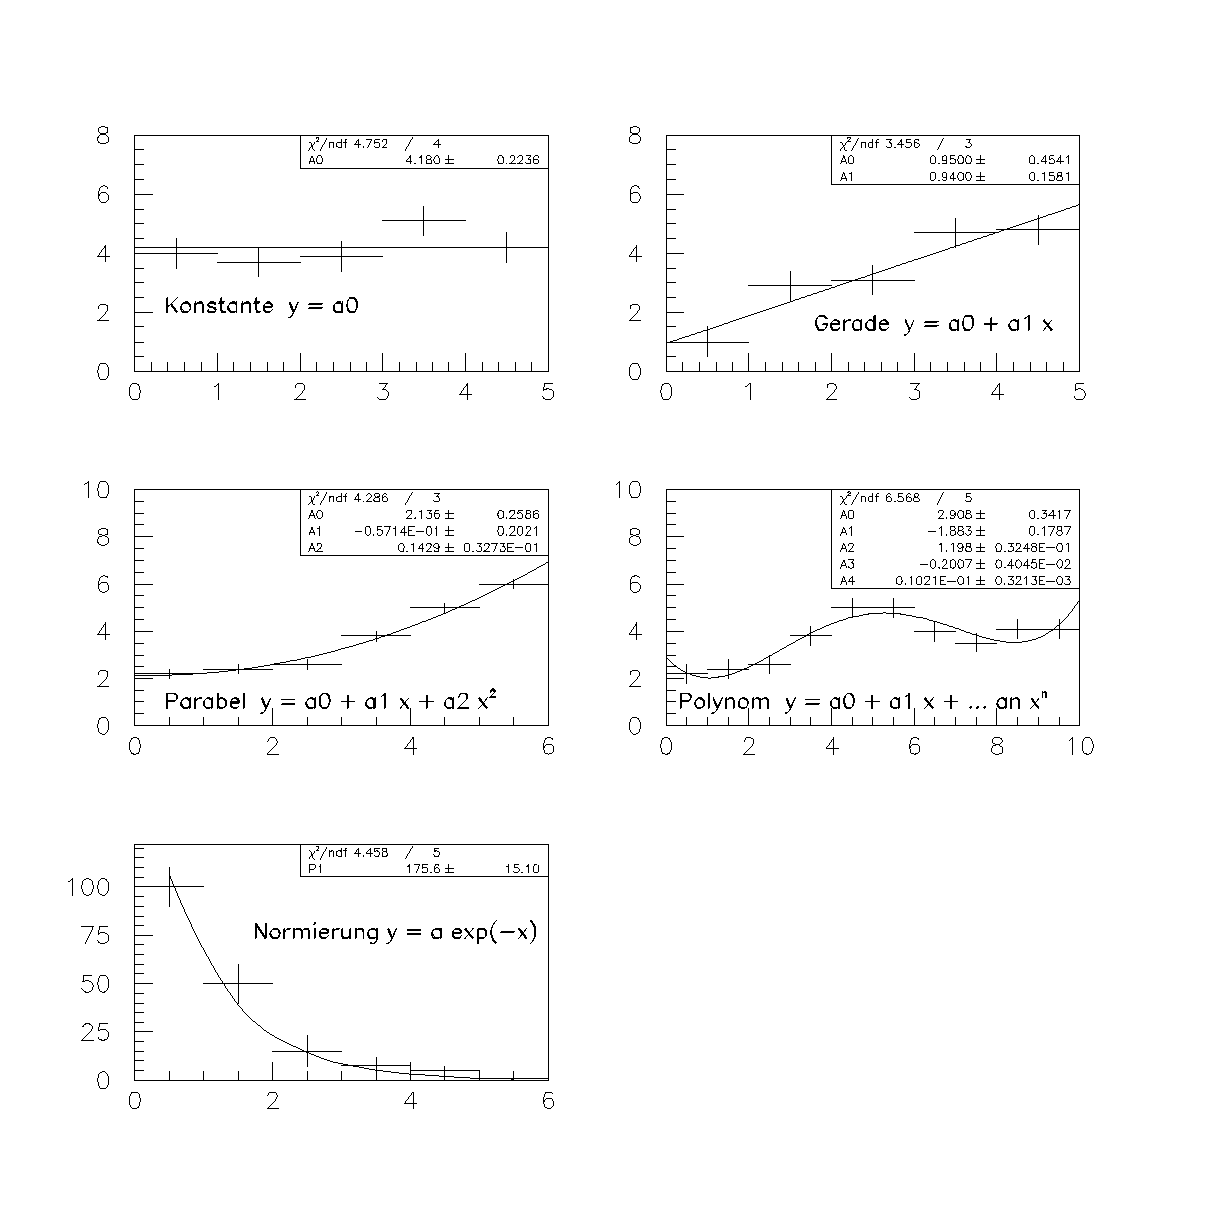
\epsfig{file=eps/linfits.eps,width=22.cm}}
\end{picture}
\end{figure}

%\section{Fit of a constant}
\Large 
Example: Averaging of different measurements 
$a_i \pm \sigma_i$ of an observable $a$ (e.g. $a = \alpha_s(m_Z)$)
\[ \chi^2 = \Sigma_i^n \frac{ (a_i - a)^2}{\sigma_i^2} \]

``Idiot'' example of one single measurement $a_1 \pm \sigma_1$:
\[ \chi^2 = \frac{ (a_1 - a)^2}{\sigma_1^2} \]
\[Min. \chi^2: \quad \frac{d \chi^2}{da} = \; 
\rightarrow \; \mbox{Estimated value}\quad
\hat{a} = a_1; \; \sigma_{\hat{a}} = \sigma_1 \]
%
Probability density $p$ for true value of $a$ ({\em inverse probability}):
\[ p \sim e^{-\chi^2/2} = 
e^{- \frac{(a - \hat{a})^2}{2\sigma_{\hat{a}}^2}} \]
%
Important relation:
\[ \sigma_{\hat{a}} = \left[ -\frac{d\chi^2}{da^2} \right]^{-1/2}
\]

\begin{figure}[h]
\unitlength1cm
  \begin{picture}(8,7.)
    \put(0.,0.){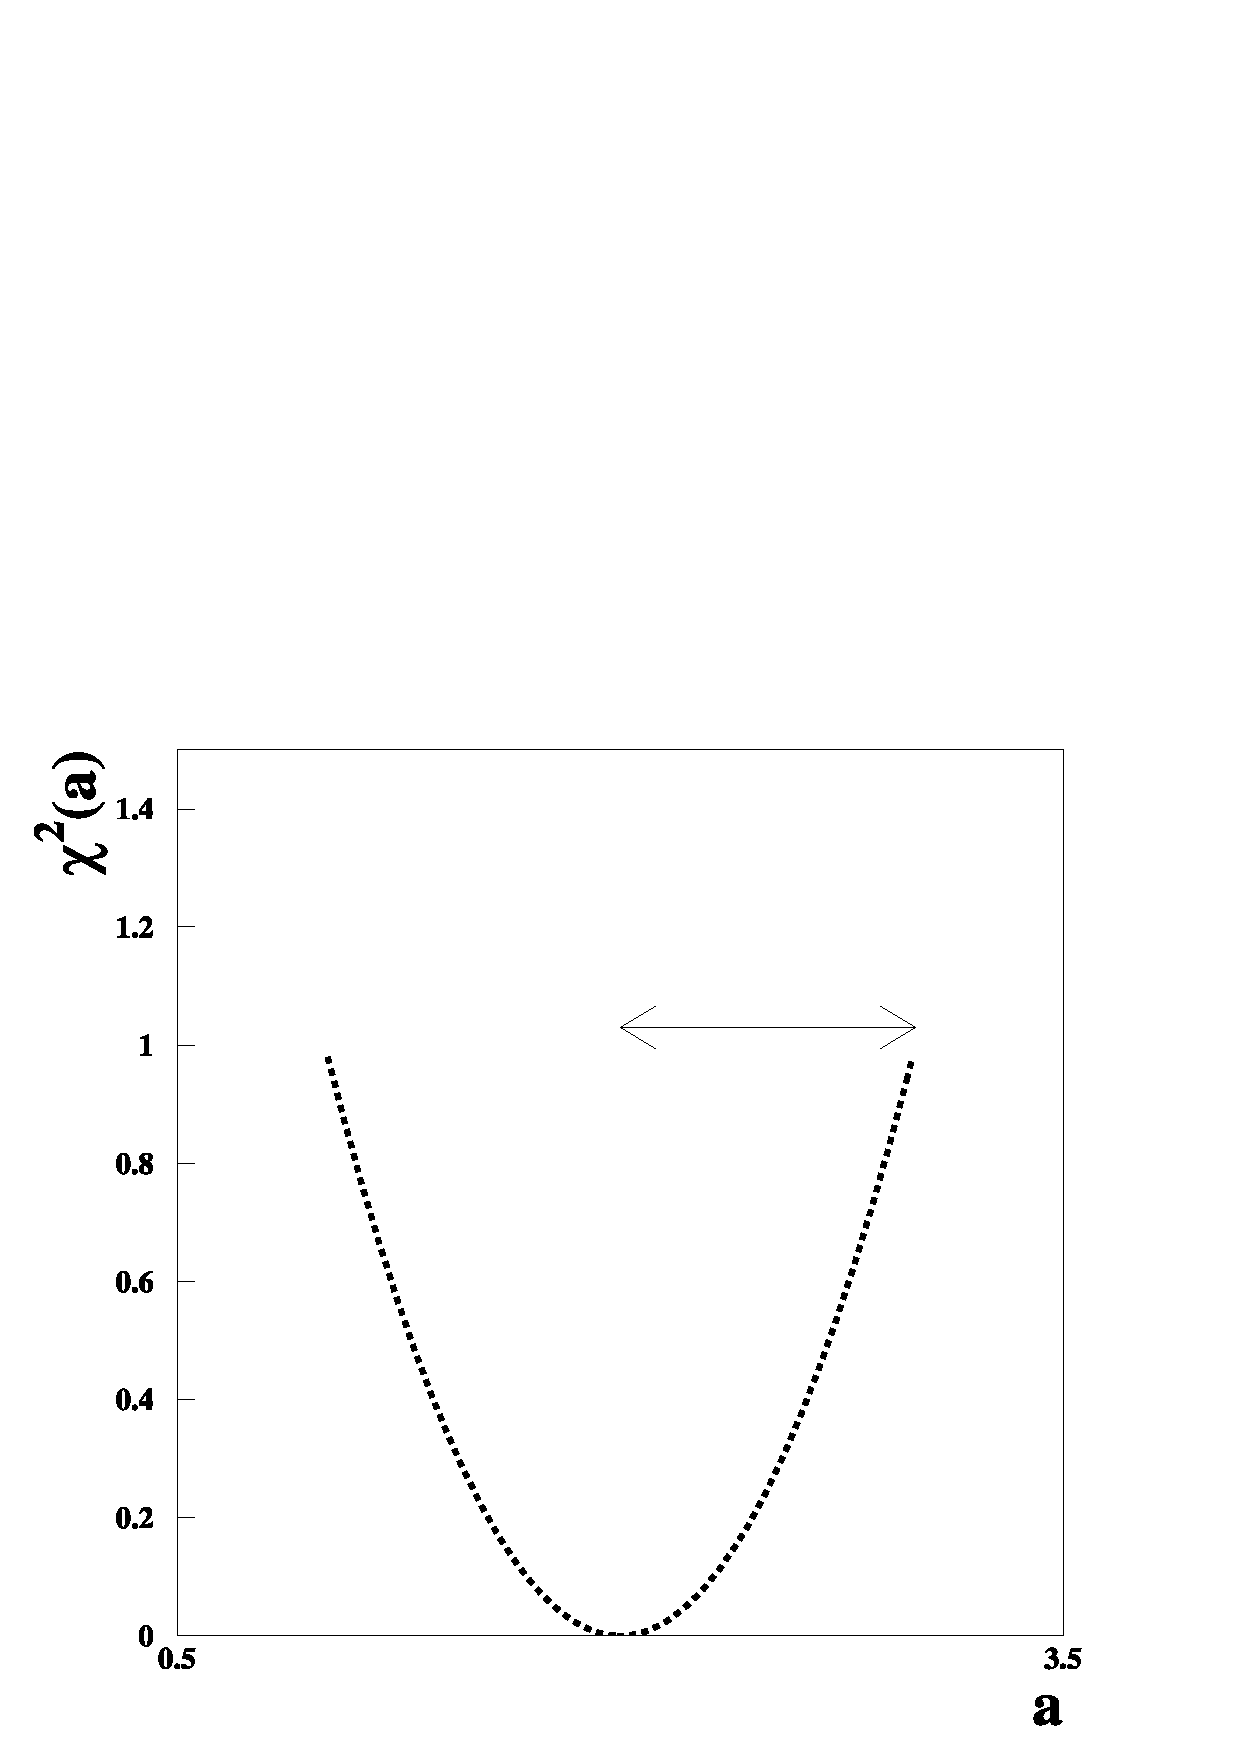
\epsfig{file=feynman/chisqp1.epsi,width=8.cm}}
    \put(8.,5.){\LARGE $\chi^2(\hat{a}+\sigma_{\hat{a}}) = 1$}
\end{picture}
\end{figure}

%\subsection{Generalisation}
\Large 
For any fit with one single parameter $a$ one finds:\\
{\em Taylor expansion} of $\chi^2$ around estimated value $\hat{a}$:
\[ 
\chi^2 = \chi^2(\hat{a}) + \frac{d\chi^2}{da_{|a=\hat{a}}} 
\cdot (a - \hat{a}) + \frac{1}{2}\, 
\frac{d^2\chi^2}{da^2_{|a=\hat{a}}}
\cdot (a - \hat{a})^2 + ...
\]
\[ = \chi^2(\hat{a}) + H \cdot (a - \hat{a})^2 \quad
\mbox{with} \quad H = \frac{1}{2}\,\frac{d^2\chi^2}{da^2_{|a=\hat{a}}}
\quad \mbox{Hesse matrix}
\]
Thus the {\em inverse probability density} is 
\[
 p(a|\hat{a}) \sim e^{-\frac{\chi^2(\hat{a})}{2}}
 \cdot 
e^{-\frac{1}{2}\, H \cdot (\hat{a}-a)^2) } 
\]
$\rightarrow$ gaussian distribution around $\hat{a}$ with
width $\sigma = H^{-1/2}$
\[ \chi^2(a) = \chi^2(\hat{a}) + 
\frac{(a-\hat{a})^2}{\sigma^2} \]
\[ \rightarrow \quad \chi^2(a \pm 1 \sigma) = \chi^2(\hat{a}) + 1 
= \chi^2_{min} + 1 
\]
$\rightarrow$ Read error directly from $\chi^2$ curve
%
%
\begin{figure}[h]
\unitlength1cm
  \begin{picture}(8,7.)
    \put(0.,0.){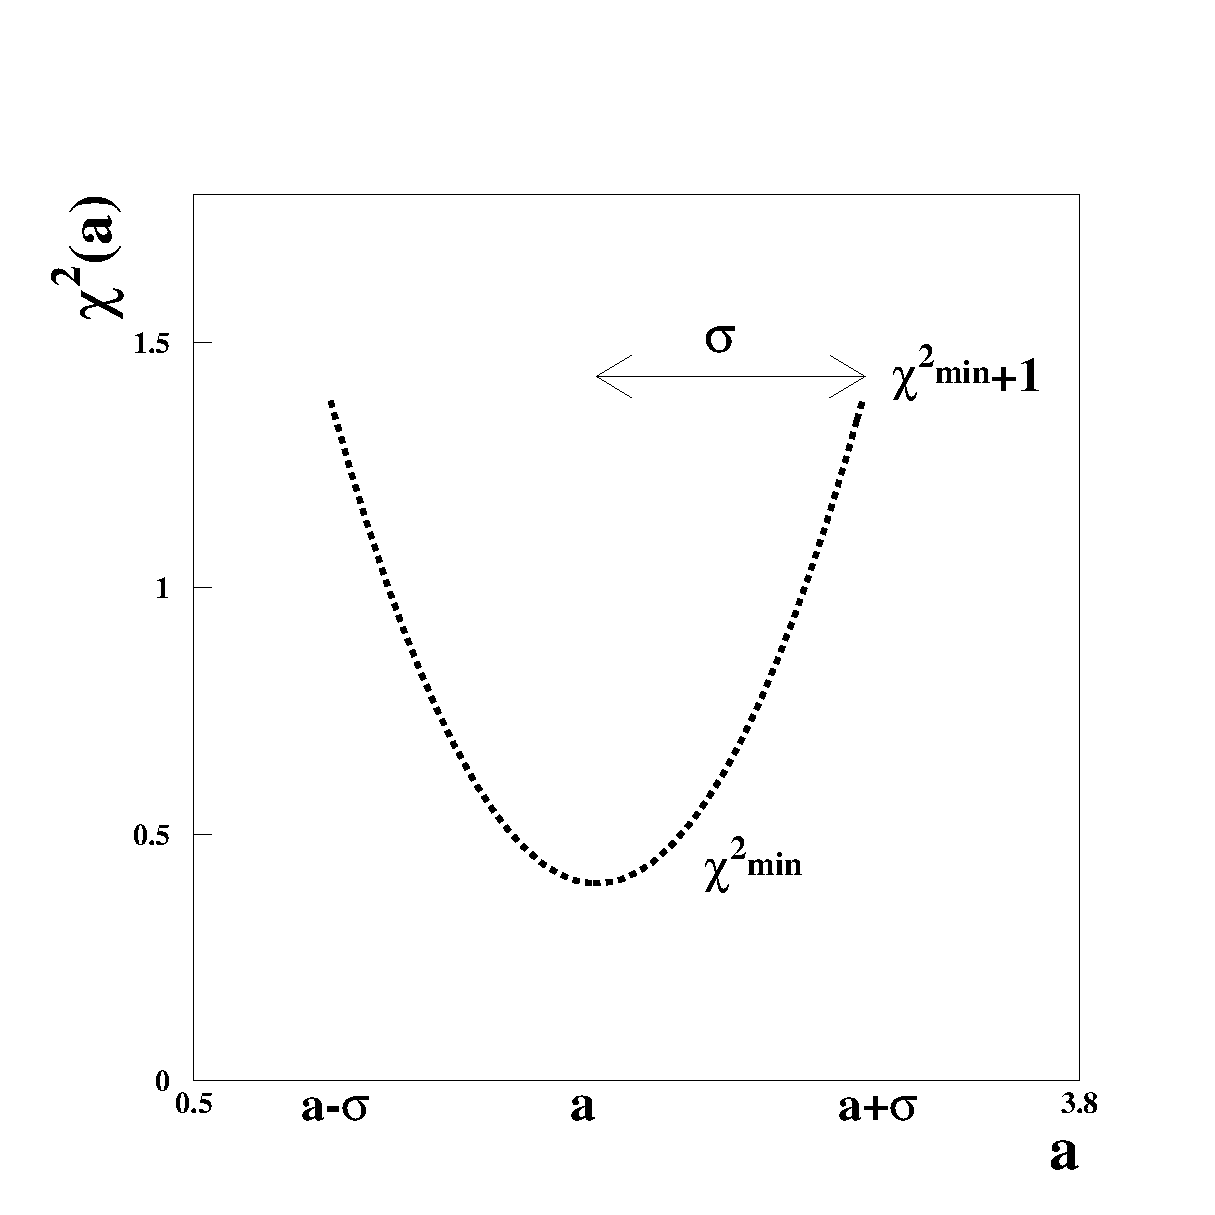
\epsfig{file=feynman/chisqp2.epsi,width=8.cm}}
%    \put(8.,5.){\LARGE $\chi^2(\hat{a}+\sigma_{\hat{a}}) = 1$}
\end{picture}
\end{figure}


%\subsection{Averaging several measurements}
%
\renewcommand{\baselinestretch}{1.1}
\Large
$n$ measurements $y_i\pm \sigma_i$ of the same quantity
$y$ $\rightarrow$ what is the best way to average?
%

\noindent
(Why is $\frac{1}{n} \Sigma y_i$ not the best? $\rightarrow$
measurements with large errors get too much weight and can
spoil the average!)
%
\[ \chi^2 = \Sigma_{i=1}^n \frac{\dd (y_i -a)^2}{\sigma_i^2} \]
%
\[ \frac{d\chi^2}{da} = 0 = \Sigma_{i=1}^{n} \frac{-2 (y_i - a)}{\sigma_i^2}
 = -2 \Sigma_{i=1}^{n} \frac{y_i}{\sigma_i^2} + 
    2 a \Sigma_{i=1}^{n} \frac{1}{\sigma_i^2}
\]
%
\[
\rightarrow \quad 
\begin{array}{|lll|}
\hline
\hat{a} & = & \Sigma_{i=1}^n \frac{\dd y_i}{\dd \sigma_i^2} /  \Sigma_{i=1}^n \frac{\dd 1}{\dd \sigma_i^2} 
\\[4mm]
\hline
\end{array}
\]
%

$\rightarrow$ Single measurements contribute with weight 
$G_i = \frac{\dd 1}{\dd \sigma_i^2}$; 

Define $G_s:= \Sigma_{i=1}^{n} G_i$ 

Hesse Matrix $H = 1/2 \frac{\dd d^2\chi^2}{\dd da^2} = G_s$
%
 
\[
\rightarrow \quad 
\begin{array}{|lll|}
\hline
\hat{a} & = & \frac{1}{\Sigma_{i=1}^n G_i}  \cdot 
\Sigma_{i=1}^n G_i y_i = \frac{1}{G_s} \cdot \Sigma_{i=1}^n G_i y_i
\\[2mm]
\hline
\end{array}
\]
%
Error on $\hat{a}$: 
%
\[ 
\begin{array}{|l|}
\hline
\sigma_{\hat{a}}^2 = \Sigma_{i=1}^n \left( \frac{\dd d\hat{a}}{\dd dy_i}\right)^2 
\cdot \sigma_i^2 = 
\Sigma_{i=1}^n \left( \frac{\dd G_i}{\dd G_s}\right)^2 
\cdot \sigma_i^2 \\
= 
\frac{\dd 1}{\dd G_s^2} \cdot \Sigma_{i=1}^n G_i = \frac{\dd 1}{\dd G_s} = 
\frac{\dd 1}{\dd \Sigma_{i=1}^n 1/\sigma_i^2} 
\\[4mm]
\hline
\end{array}
\]

In short
\[ 
\begin{array}{|l|}
\hline
\hat{a} = \frac{ \dd \Sigma_{i=1}^n y_i/\sigma_i^2}{\dd
 \Sigma_{i=1}^n 1/\sigma_i^2} \; \pm \; \frac{\dd 1}{\dd 
\sqrt{\Sigma_{i=1}^n 1/\sigma_i^2} }
\\[4mm]
\hline
\end{array}
\]





%\begin{slide}
\Large
\pagestyle{headings}
\sf
\header{Solution via normal equations}
Linear fit $\rightarrow$ determines estimator for $\vec{a}$
\[ \chi^2 = (\vec{y} - A\vec{a})^{t} V^{-1} 
            (\vec{y} - A\vec{a}) \]
\[Min. \chi^2 \;\rightarrow \;\frac{d\chi^2}{d\vec{a}^{\,t}}  = 0 \]
\[ \rightarrow \;-2 A^t V^{-1} (\vec{y} - A \vec{a}) = 0
\]
\[ \rightarrow \; A^t V^{-1} A \vec{a} = A^{t} V^{-1} \vec{y} \]

\noindent
{\em Side remark: why can't we just set: 
$\vec{y} = A \vec{a}$ ??? Because 
$\vec{y}$ has dimension
$n$ and $\vec{a}$ has dimension $m$ !!!
}
\noindent
\underline{Solution:}
\[ 
\begin{array}{||lll||} 
\hline
\hline
\vec{a} &  = &   (A^t V^{-1} A)^{-1} A^t V^{-1} \vec{y}  \\
 & = & H^{-1} A^t V^{-1} \vec{y} \\
 & = & U A^t V^{-1} \vec{y} \\
 & & \mbox{with}\; U= H^{-1} = Cov(a) \\ 
\hline
\hline
\end{array}
\quad
\mbox{\blue \em Normal equations}
\]
%
%
\end{slide} 


%
\end{document}
